
\begin{figure}[!ht]\centering
	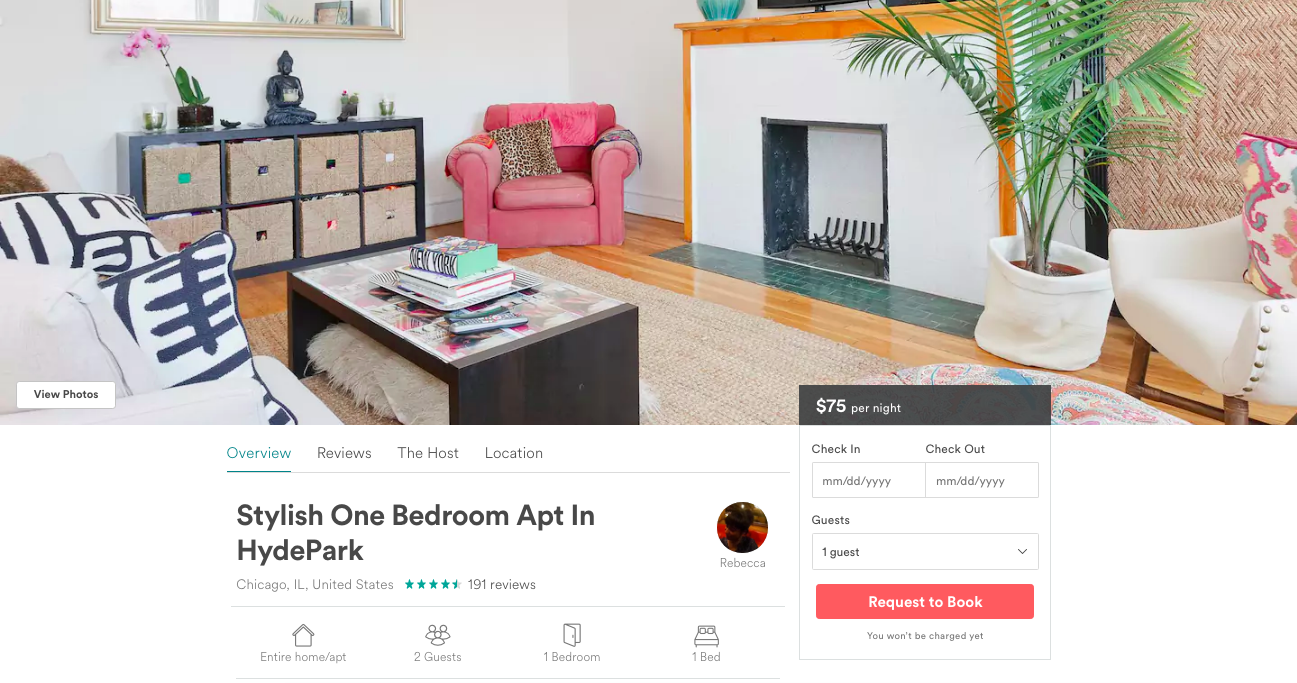
\includegraphics[width=.8\textwidth]{figures/cover}
	\caption{Sample listing page}
	\label{fig:listing}
\end{figure}

\begin{figure}[!ht]\centering
	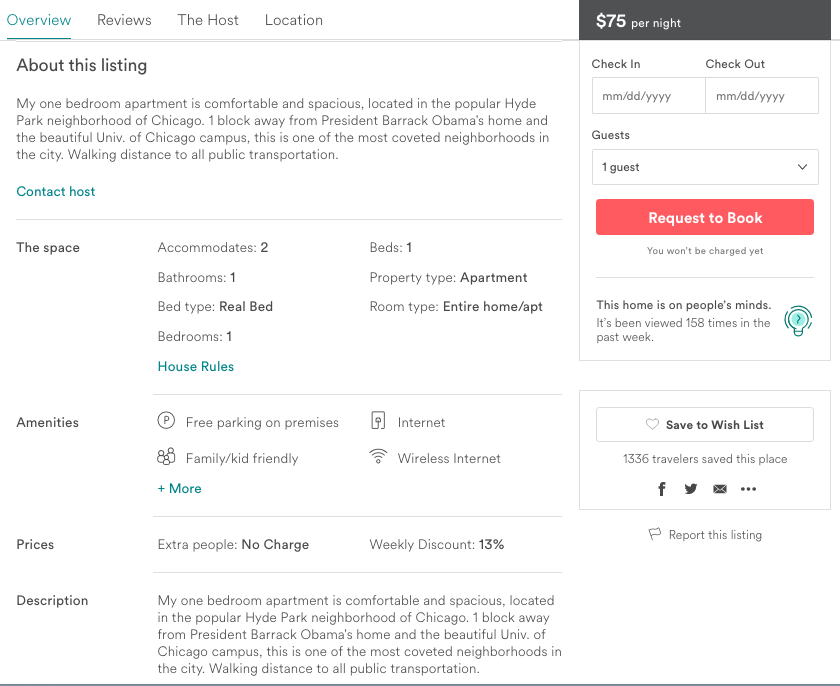
\includegraphics[width=.8\textwidth]{figures/property}
	\caption{Listing information}
	\label{fig:property}
\end{figure}

\begin{figure}\centering
	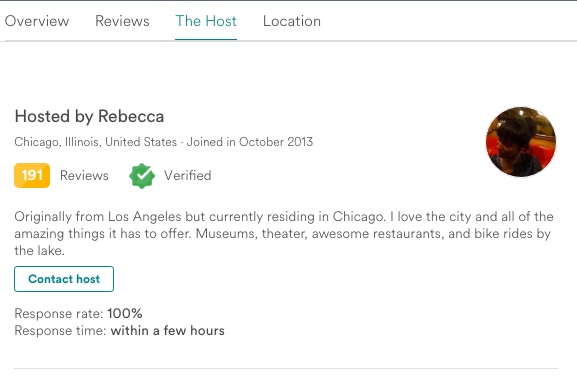
\includegraphics[width=.9\textwidth]{figures/host}
	\caption{Host information}
	\label{fig:host}
\end{figure}

\begin{figure}\centering
	\includegraphics[width=.8\textwidth]{figures/chicago_city_neighborhoods}
	\caption[City of Chicago neighborhoods]{City of Chicago neighborhoods, showing level of granularity of neighborhood controls}
	\label{fig:chicago}
\end{figure}

\begin{figure}\centering
	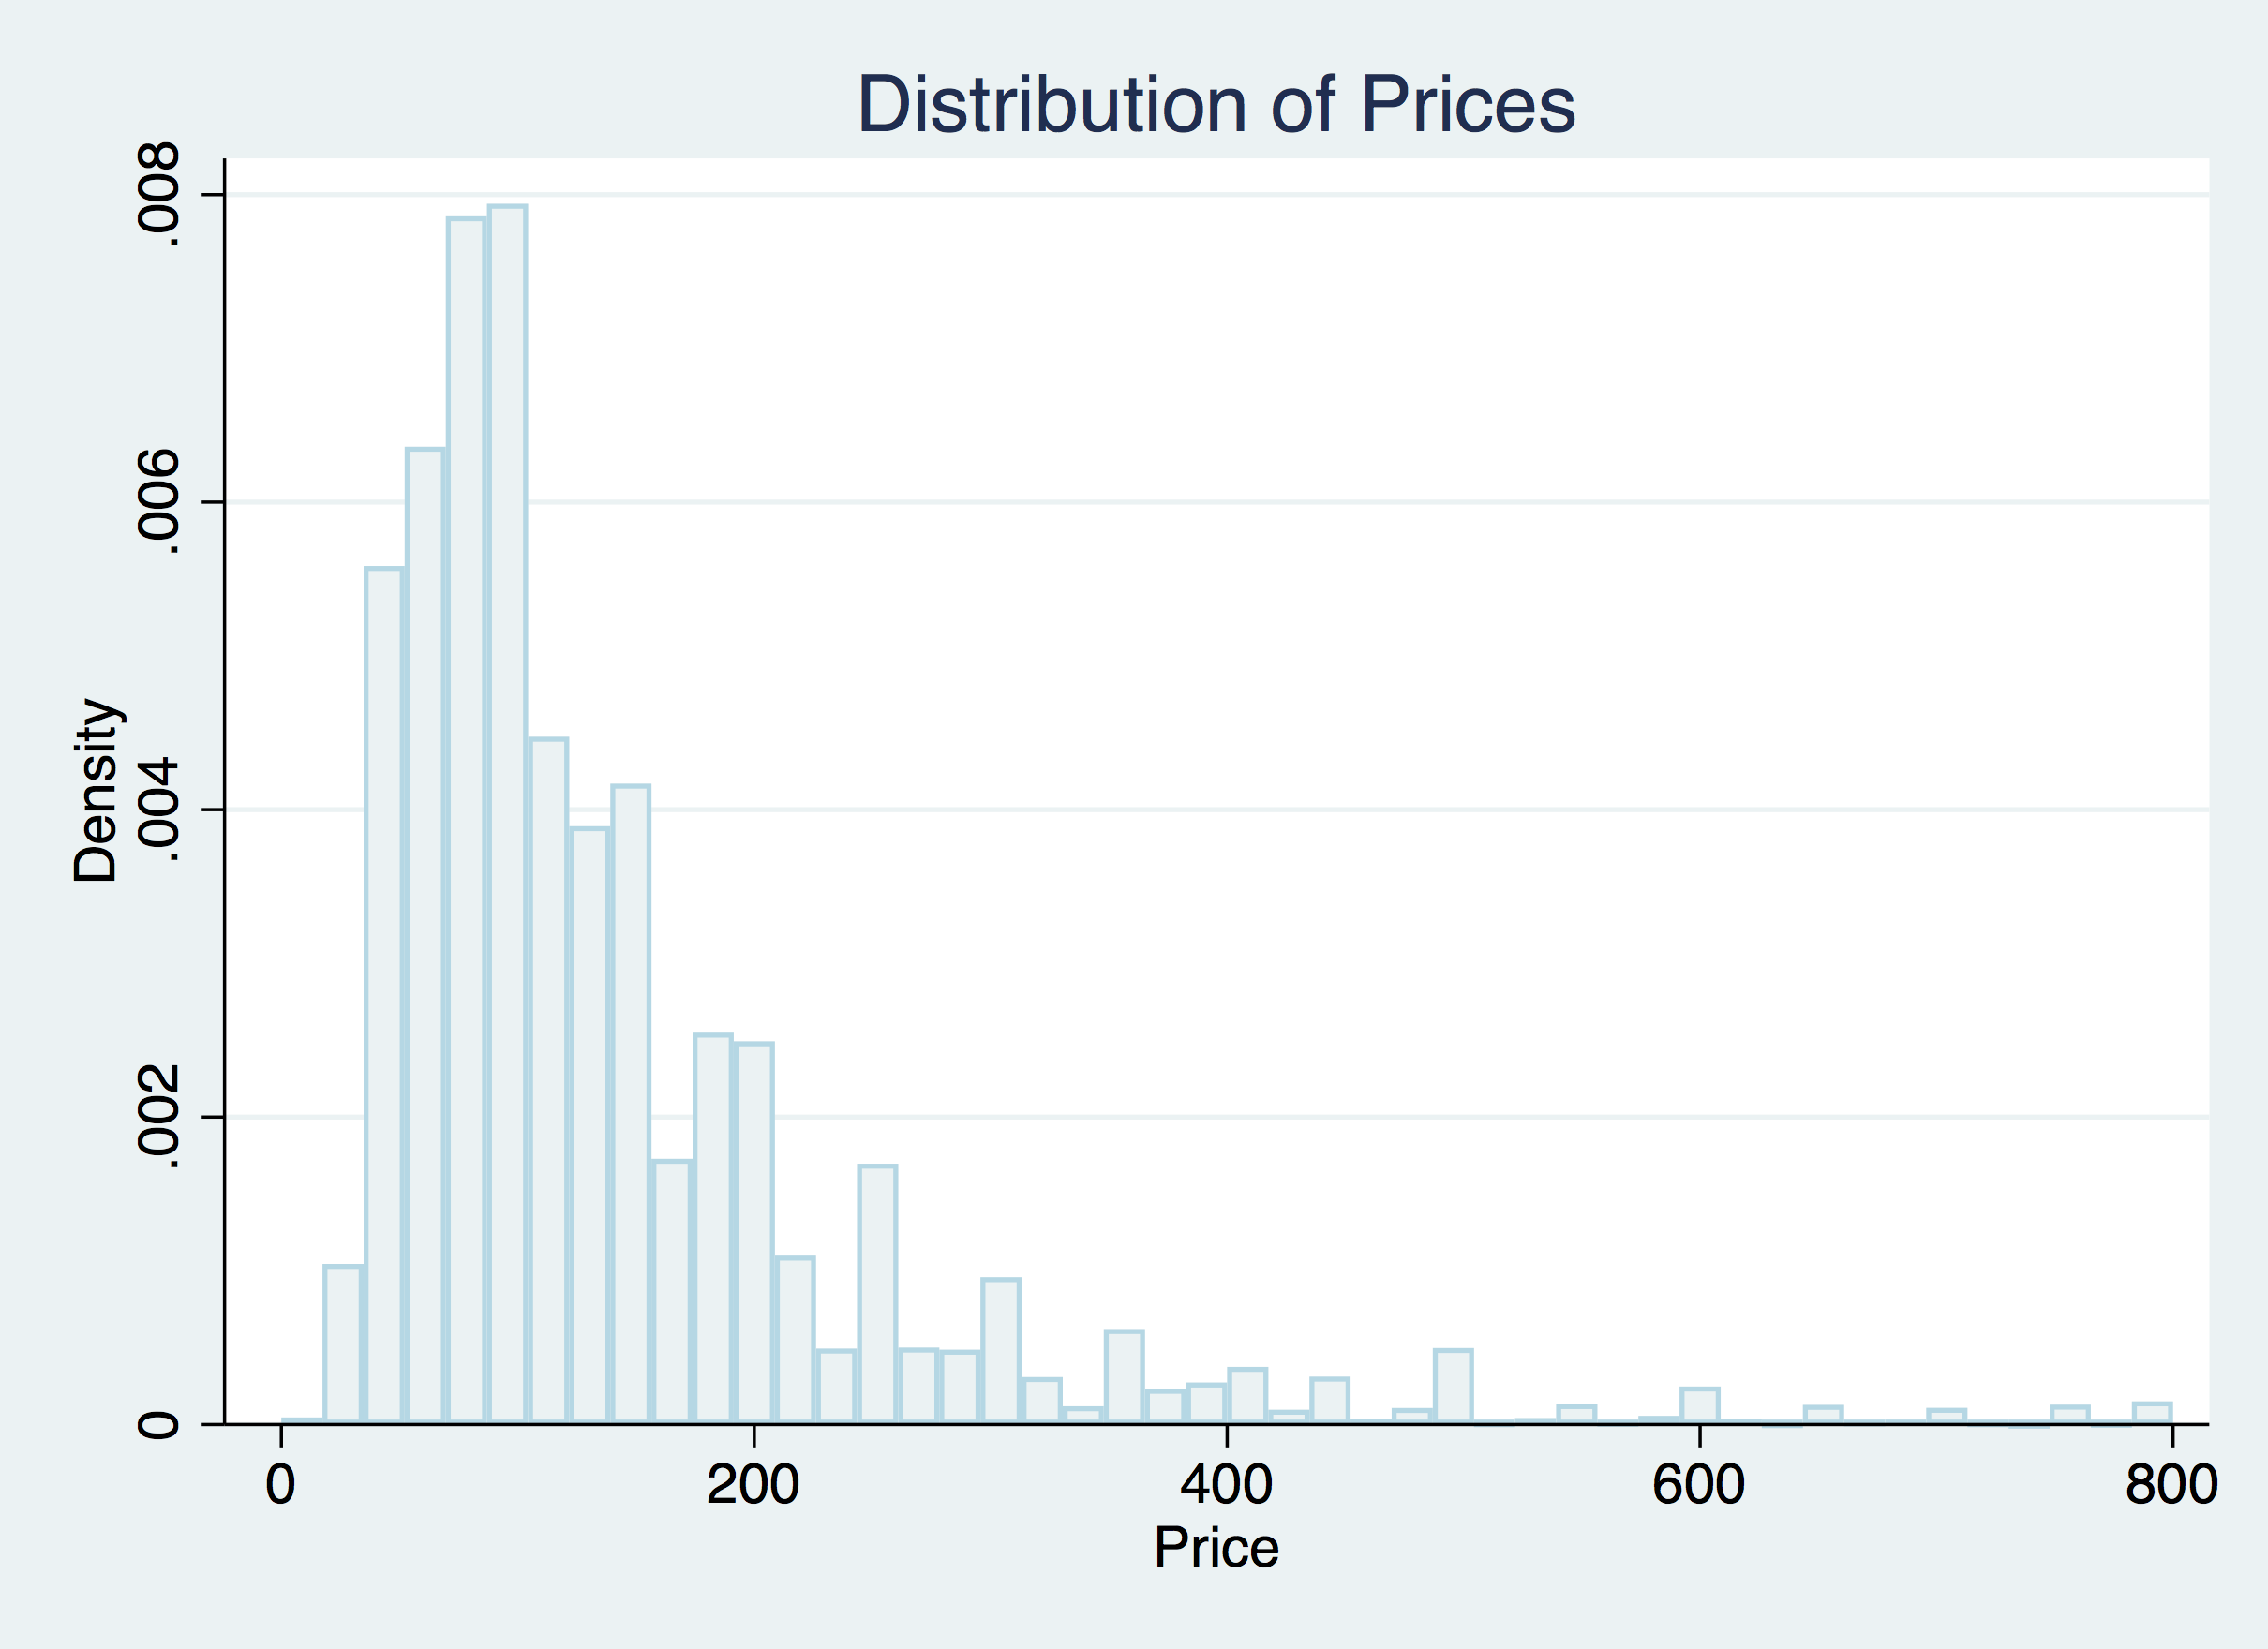
\includegraphics[width=.9\textwidth]{figures/fig1_price}
	\caption{Distribution of listing prices in the sample}
	\label{fig:prices}
\end{figure}

\begin{figure}\centering
	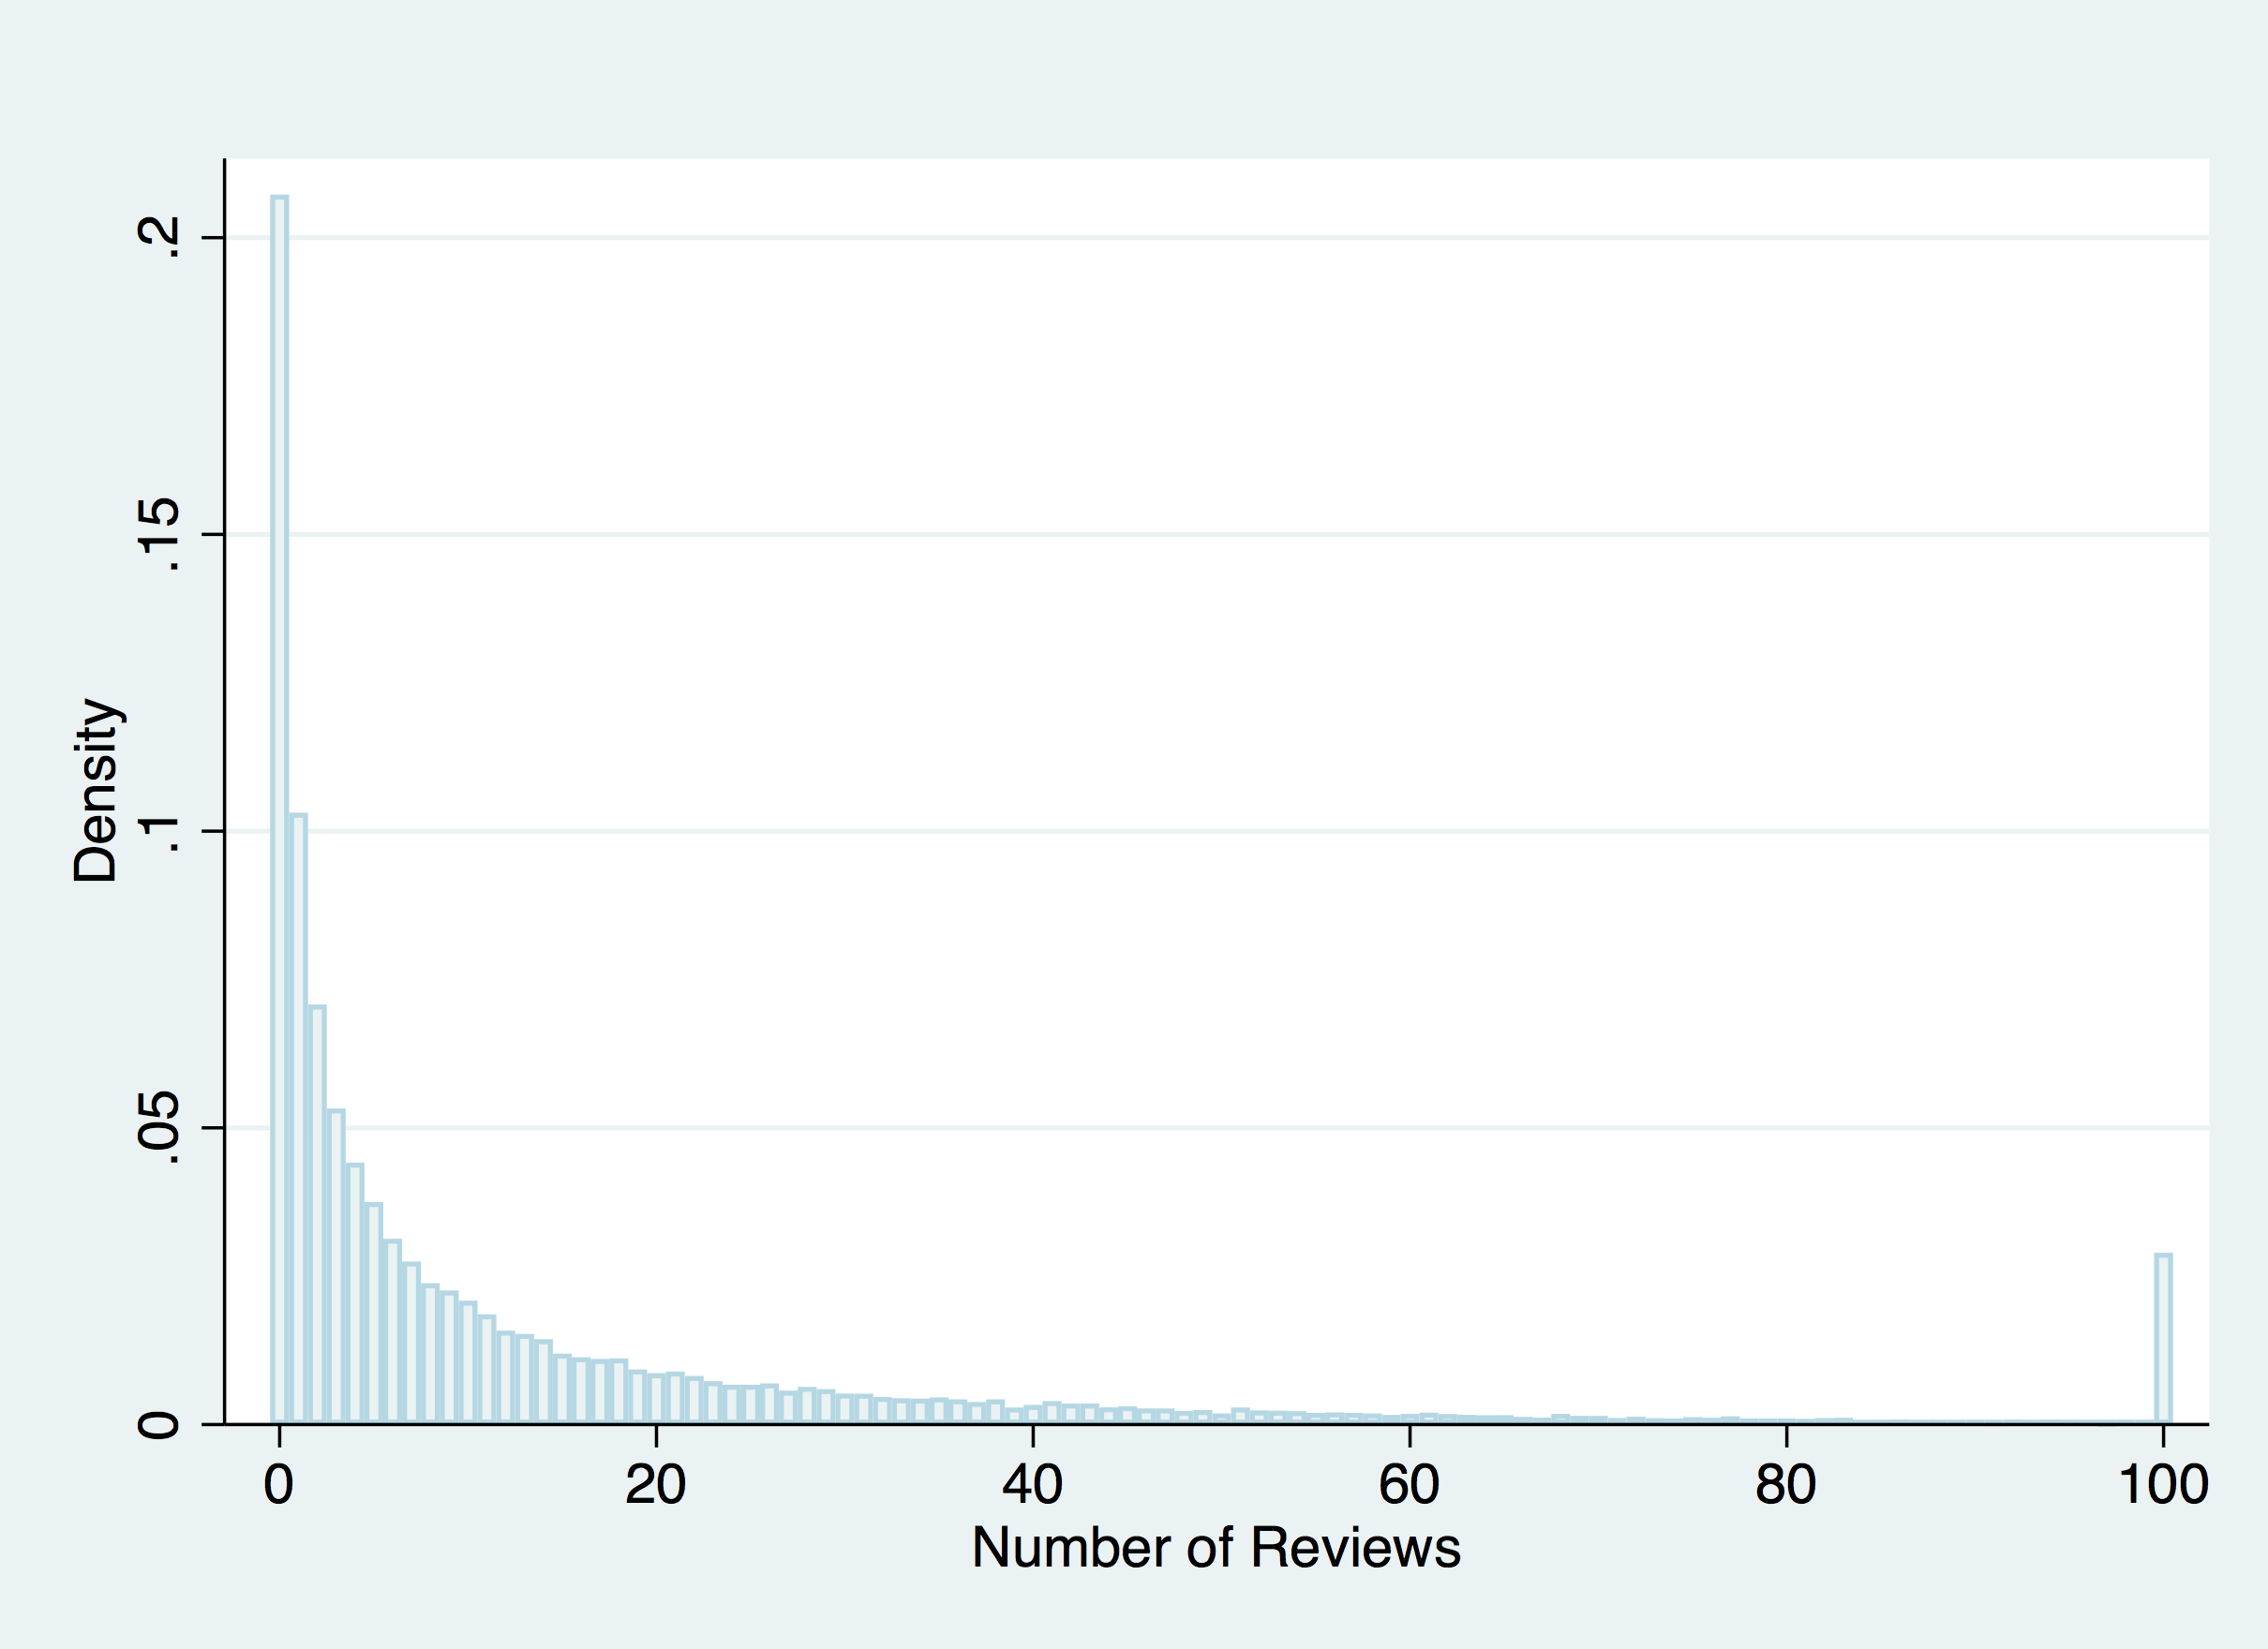
\includegraphics[width=.8\textwidth]{figures/fig2_num_reviews}
	\caption{Distribution of the number of reviews per listing}
	\label{fig:num_reviews}
\end{figure}

\begin{figure}\centering
	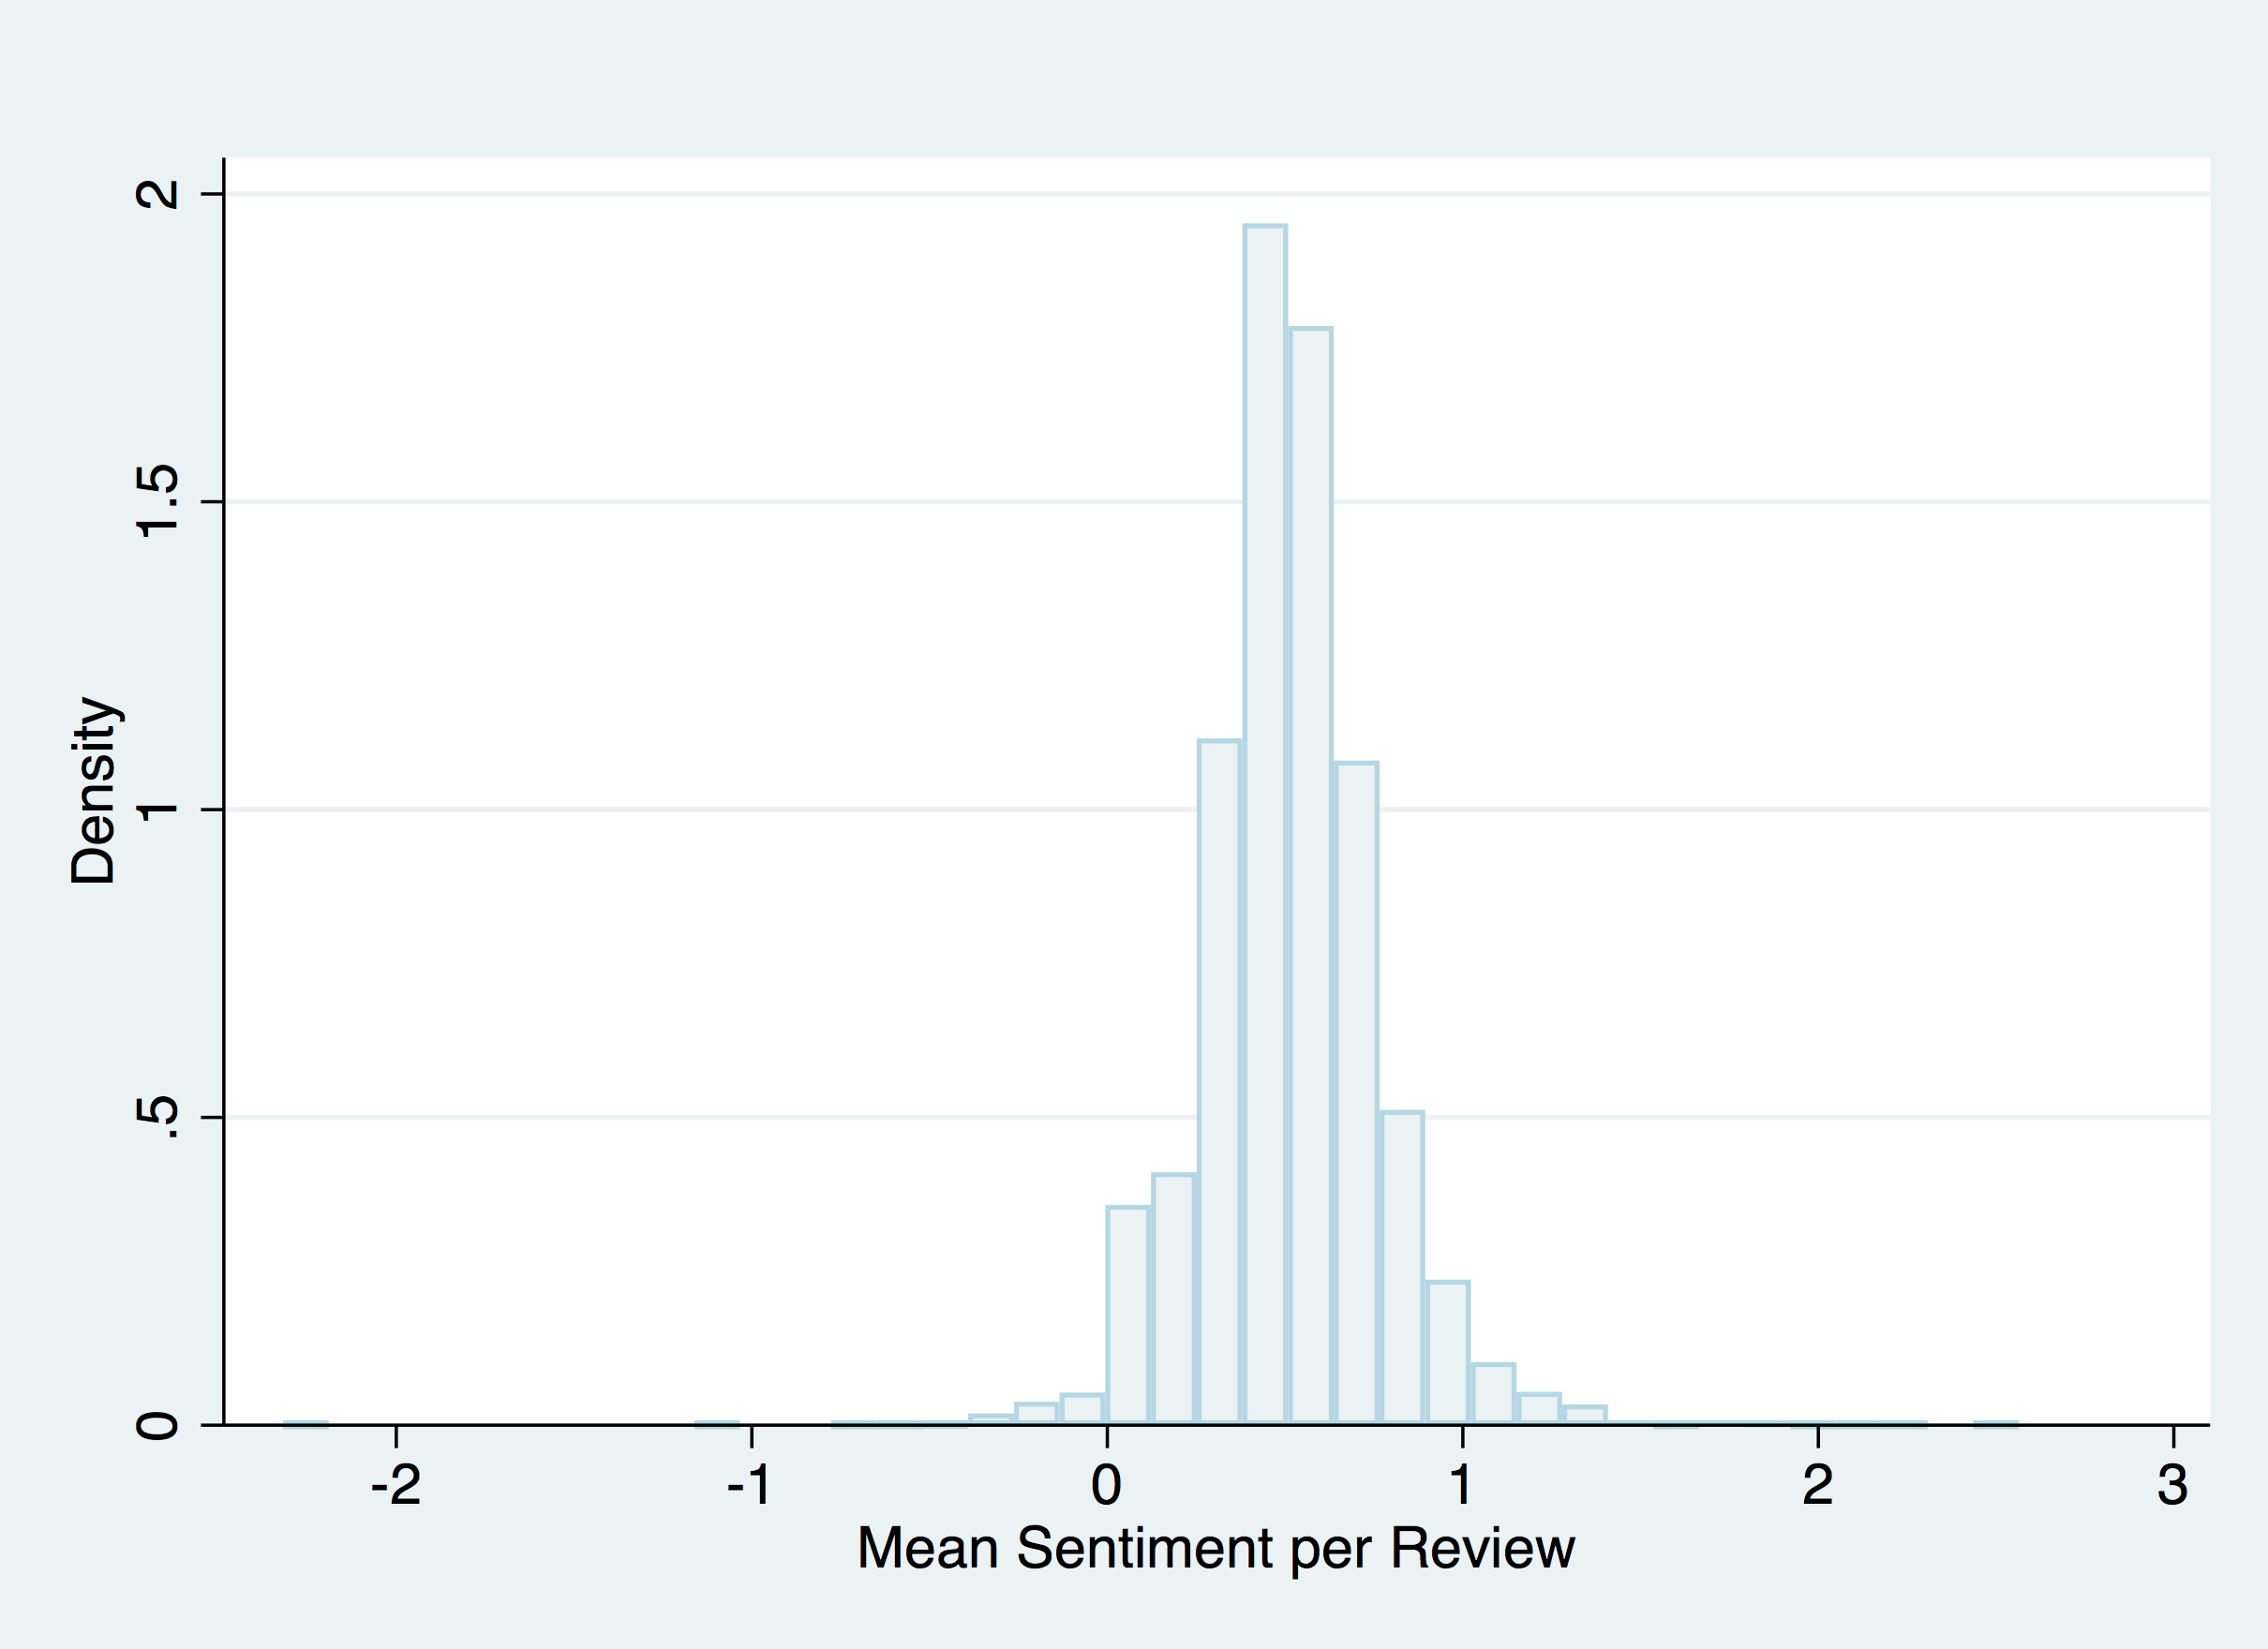
\includegraphics[width=.8\textwidth]{figures/fig3_review_sentiment}
	\caption{Distribution of average review sentiment per listing}
	\label{fig:sentiment}
\end{figure}

% is this ever used? 

\begin{comment}
\begin{figure}[!ht]\centering
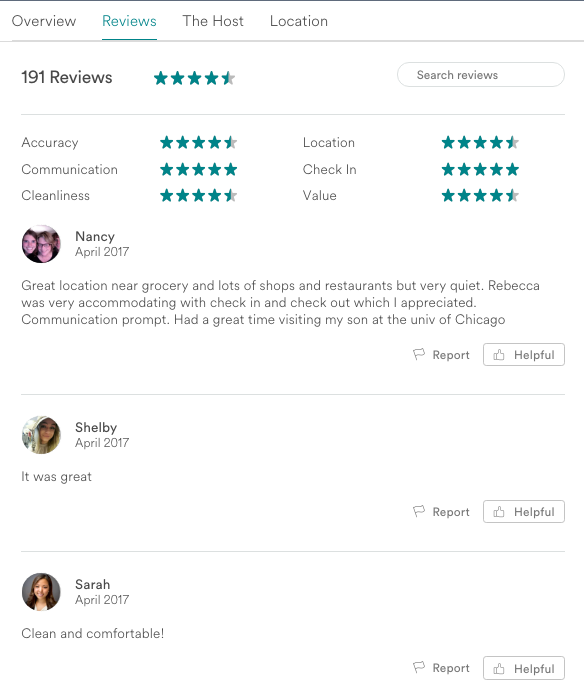
\includegraphics[width=.8\textwidth]{figures/reviews}
\caption{Review information}
\label{fig:reviewinfo}
\end{figure}


\begin{figure}\centering
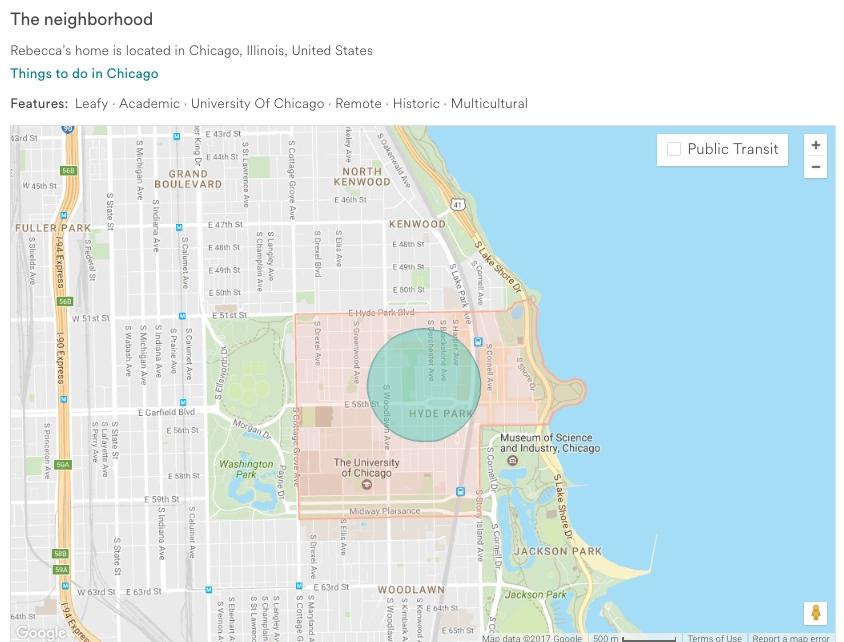
\includegraphics[width=.8\textwidth]{figures/location}
\caption{Location information}
\label{fig:location}
\end{figure}
\end{comment}



